\chapter{Arquitectura del Sistema e Ingesta (Capa Bronze)}

\section{Arquitectura Cloud Always Free y patrón Medallion}
El sistema ha sido diseñado bajo una premisa de coste operativo nulo en almacenamiento y análisis (\textit{Always Free}), evitando tarifas de transferencia (\textit{egress}) mediante \textbf{Cloudflare R2} (compatible con la API S3 Signature v4) y aplicando la arquitectura \textbf{Medallion}:

\begin{itemize}
    \item \textbf{Capa Bronze (\texttt{raw/}):} Datos inmutables en formato columnar Parquet con compresión \texttt{ZSTD} (y artefactos crudos preservados con esquema en lectura).
    \item \textbf{Capa Silver (\texttt{silver/}):} Registros depurados, normalizados al huso horario \texttt{America/New\_York}, filtrados por el \textit{Gatekeeper} semántico y enriquecidos con puntuaciones de sentimiento.
    \item \textbf{Capa Gold (\texttt{gold/}):} Matrices tabulares unificadas $(X_t \rightarrow y_{t+1})$ listas para entrenamiento, inferencia y consumo desde el cuadro de mando.
\end{itemize}

% Ejemplo para insertar el diagrama de arquitectura cuando se copie a figures/
% \begin{figure}[H]
%     \centering
%     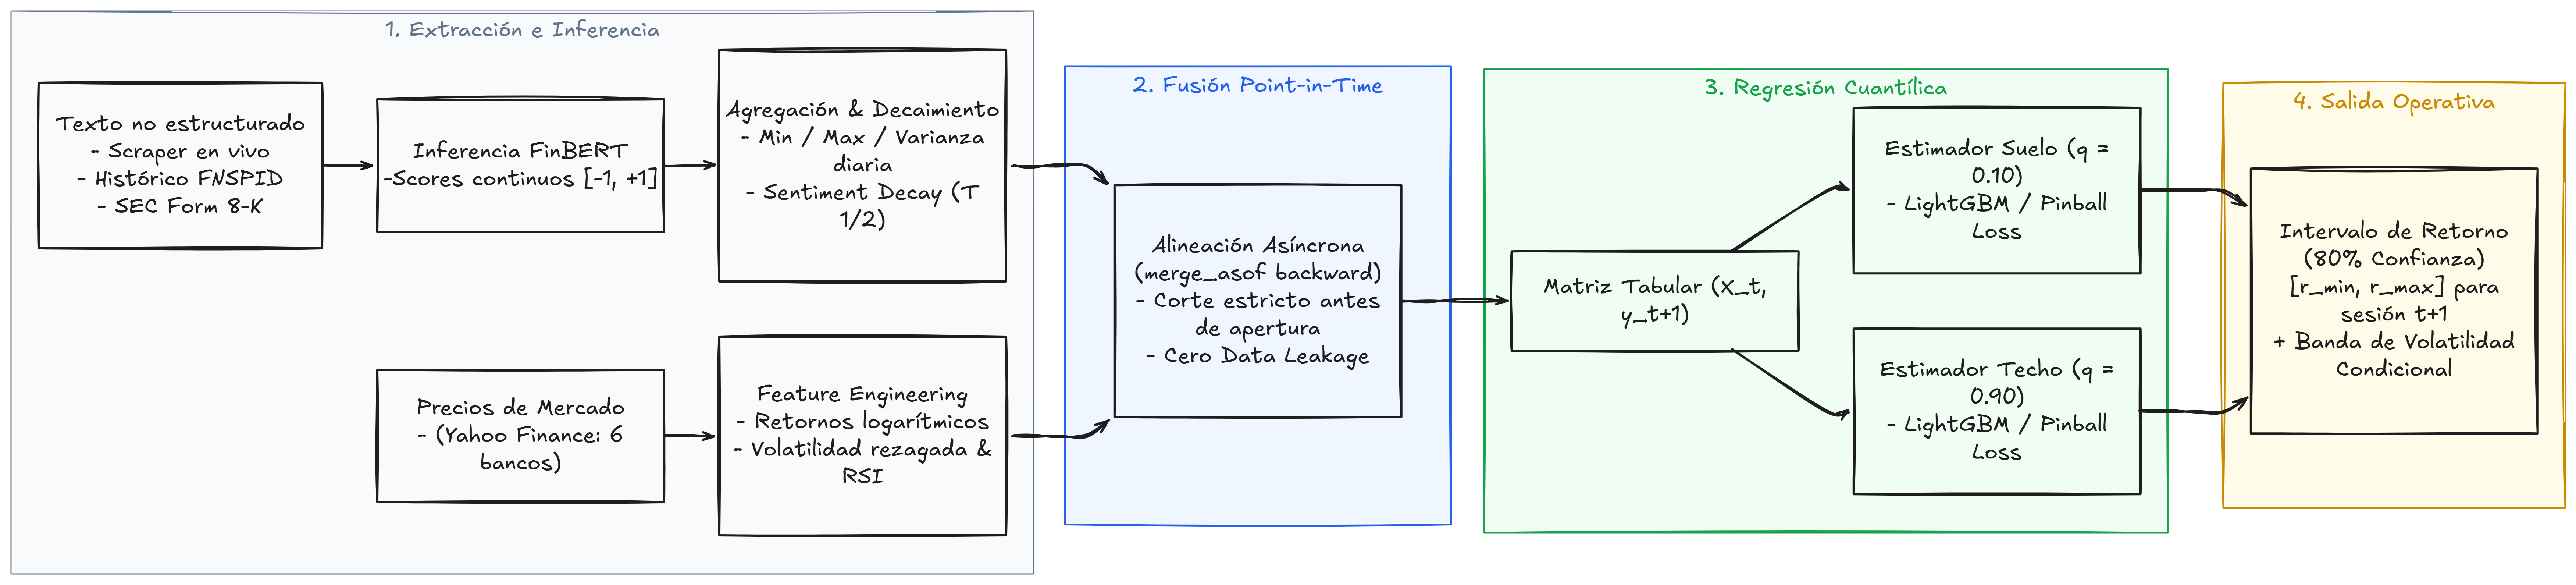
\includegraphics[width=0.95\textwidth]{diagrama-de-tfm-predecir-la-bolsa.png}
%     \caption{Arquitectura integral del flujo de datos multimodal (Bronze, Silver y Gold).}
%     \label{fig:arquitectura_medallion}
% \end{figure}

\section{Universo bancario y catálogo canónico}
La fuente única de verdad para los seis bancos del estudio reside en \texttt{src/shared/tickets.py}, centralizando \textit{tickers}, códigos CIK oficiales de la SEC y alias semánticos para evitar colisiones léxicas:

\begin{table}[H]
    \centering
    \caption{Universo bancario US Big 6 y cobertura consolidada en Capa Bronze (2010--2023).}
    \label{tab:universo_big6}
    \begin{tabular}{@{}llrr@{}}
        \toprule
        \textbf{Ticker} & \textbf{Entidad financiera} & \textbf{CIK SEC} & \textbf{Noticias Bronze} \\
        \midrule
        \texttt{JPM} & JPMorgan Chase \& Co.        & \texttt{0000019617} & 18.953 \\
        \texttt{BAC} & Bank of America Corp.        & \texttt{0000070858} & 11.509 \\
        \texttt{WFC} & Wells Fargo \& Company       & \texttt{0000072971} & 16.075 \\
        \texttt{C}   & Citigroup Inc.               & \texttt{0000831001} &  8.647 \\
        \texttt{GS}  & Goldman Sachs Group Inc.     & \texttt{0000886982} & 18.321 \\
        \texttt{MS}  & Morgan Stanley               & \texttt{0000895421} & 16.341 \\
        \midrule
        \textbf{Total} & \textbf{6 entidades} & --- & \textbf{89.846} \\
        \bottomrule
    \end{tabular}
\end{table}

\section{Fuentes de datos e ingesta multimodal (2010--2023)}
\begin{itemize}
    \item \textbf{Cotizaciones bursátiles (\texttt{src/mercado/yfinance\_extractor.py}):} Descarga histórica ajustada por \textit{splits} y dividendos (\texttt{auto\_adjust=True}) consolidada en el archivo \texttt{raw/yfinance/\allowbreak stocks\_2010\_2023.parquet}.
    \item \textbf{Eventos regulatorios SEC EDGAR (\texttt{src/sec/}):} Descubrimiento mediante API REST oficial respetando la política \textit{Fair Access} ($\le 10$ req/s). Se consolidaron tres conjuntos en R2: \texttt{8k-2010-2023.parquet} (5.424 ítems en 2.903 \textit{filings} únicos), \texttt{8k-exhibits-2010-2023.parquet} (5.531 anexos \texttt{EX-*} en 2.324 \textit{filings}, excluyendo XBRL técnicos \texttt{EX-101.*}, según ADR-007) y \texttt{10k-10q-2010-2023.parquet} (336 \textit{filings}).
    \item \textbf{Noticias financieras (\texttt{src/articulos/etl\_multisource.py}):} Procesamiento \textit{pushdown} con DuckDB sobre 21,4\,GB crudos (\textit{financial-news-multisource}), desacoplando \texttt{title} y \texttt{article}, normalizando fechas a \texttt{America/New\_York} con trazabilidad de sesión (\texttt{premarket}, \texttt{intraday}, \texttt{afterhours}, \texttt{date\_only}) y generando \texttt{raw/huggingface/multisource\_bancos\_2010\_2023.parquet} (89.846 registros tras deduplicación canónica).
\end{itemize}

\section{Diseño modular, Clean Architecture y cumplimiento normativo}
El código fuente sigue una separación estricta en capas (\textit{Dominio}, \textit{Casos de Uso/ETLs}, \textit{Infraestructura} e \textit{Inyección de Dependencias} en \texttt{src/dependencies/}), reutilizando de forma centralizada la compactación columnar en memoria (\texttt{ParquetCompactor} con PyArrow \texttt{ZSTD}) y el repositorio asíncrono S3/R2 (\texttt{S3StorageRepository}). Asimismo, el sistema cumple un diseño \textit{Compliance-by-Design} amparado en la excepción de minería de textos con fines académicos (Directiva UE 2019/790, Art.~3), inferencia efímera y ausencia total de datos personales (exención RGPD).
